% CVPR 2025 Paper Template; see https://github.com/cvpr-org/author-kit

\documentclass[10pt,twocolumn,letterpaper]{article}

%%%%%%%%% PAPER TYPE  - PLEASE UPDATE FOR FINAL VERSION
\usepackage[pagenumbers]{cvpr} % To force page numbers, e.g. for an arXiv version

% Import additional packages in the preamble file, before hyperref
%
% --- inline annotations
%
\usepackage[dvipsnames]{xcolor}
\newcommand{\red}[1]{{\color{red}#1}}
\newcommand{\todo}[1]{{\color{red}#1}}
\newcommand{\TODO}[1]{\textbf{\color{red}[TODO: #1]}}
% --- disable by uncommenting  
% \renewcommand{\TODO}[1]{}
% \renewcommand{\todo}[1]{#1}



% It is strongly recommended to use hyperref, especially for the review version.
% hyperref with option pagebackref eases the reviewers' job.
% Please disable hyperref *only* if you encounter grave issues,
% e.g. with the file validation for the camera-ready version.
%
% If you comment hyperref and then uncomment it, you should delete *.aux before re-running LaTeX.
% (Or just hit 'q' on the first LaTeX run, let it finish, and you should be clear).
\definecolor{cvprblue}{rgb}{0.21,0.49,0.74}
\usepackage[pagebackref,breaklinks,colorlinks,allcolors=cvprblue]{hyperref}

\def\confName{COMPSCI68@UMass}
\def\confYear{2024}

%%%%%%%%% TITLE - PLEASE UPDATE
\title{Generative Adversarial Networks for Galaxy Classification Using Convolutional
Neural Networks}

%%%%%%%%% AUTHORS - PLEASE UPDATE
\author{Polina Petrova\\
{\tt\small ppetrova@umass.edu}
\and
Aryan Singh\\
{\tt\small arysingh@umass.edu}
}

\begin{document}
\maketitle
% ABSTRACT
\begin{abstract}
    The classification of galaxies poses significant challenges due to inherent data imbalances among various morphological classes. 
    This research addresses the pressing issue of accurately classifying galaxies using Convolutional Neural Networks (CNNs), where traditional approaches often struggle with underrepresented categories. 
    To mitigate this problem, we propose a novel combined model utilising a Conditional Generative Adversarial Network (cGAN) to generate synthetic images that augment the Galaxy Zoo 2 dataset, which contains approximately 270,000 labelled galaxy images. 
    Our methodology begins with enhancing image resolution using Super Resolution GANs (SRGAN), followed by training the cGAN to produce additional samples for each class, thereby addressing class imbalance without resorting to deeper networks. 
    We draw on foundational works, including studies on deep generative models for galaxy image simulations and prior CNN applications in galaxy classification, to inform our approach. 
    Our model's performance will be rigorously evaluated, comparing results from training on both real and synthetic data against traditional CNNs trained on the original dataset. 
    Through this work, we aim to contribute to the ongoing efforts to improve automated galaxy classification and provide a scalable solution to the prevalent issue of data imbalance in astronomical research.
\end{abstract}

%INTRO
\section{Introduction}
With rapid development in technology comes a phenomenon that is referred to as the \textit{data deluge}, – a consequence of an overwhelming influx of data and insufficient resources to process it. 
Astronomers, in particular, contend with this challenge; estimates suggest the observable universe holds between 100 billion and 200 billion galaxies \cite{Howell2018}.
A single photograph of a small sky section can capture up to 25,000 galaxies, and the resulting daily data volume overwhelms the limited pool of experts available to classify them \cite{Sauers2023}.
To address this challenge, astrophysicists launched the \textit{Galaxy Zoo} project in 2007, inviting citizen scientists to help classify over 900,000 galaxies, marking a transformative moment in data processing through public participation \cite{McGourty2007}.

Following the success of the \textit{Galaxy Zoo}, advancements in machine learning spurred efforts to automate galaxy classification. 
Modern approaches employ Convolutional Neural Networks (CNNs) to recognise patterns with minimal human input. 
However, a persistent challenge is the quality and distribution of available data. 
While the \textit{Galaxy Zoo} project provided a substantial dataset, imbalances in class representation can skew training, causing models to favour more frequent classes. 
Our research specifically addresses this class imbalance in the Galaxy Zoo 2 dataset – a collection of categorised images taken from the Sloan Digital Sky Survey (SDSS) – where certain galaxy types are underrepresented.
Building deeper networks is a common workaround to address this issue, but we argue that this approach only sidesteps the core problem.

Ideally, a large, balanced dataset would improve model accuracy, but limitations in space imaging and classification complexity make this difficult. 
To tackle this, we propose a novel solution using Generative Adversarial Networks (GANs) to generate synthetic images for underrepresented galaxy classes in the Galaxy Zoo 2 dataset, which we then use to train a CNN. 
We expect that by augmenting our data with synthetic images, we can improve classification accuracy across all classes. 
Our evaluation will compare the GAN-CNN model's performance against traditional CNNs trained on imbalanced data, particularly examining accuracy gains in classifying underrepresented classes. 
With this combined GAN-CNN model, we aim to address class imbalance directly, eliminating the need for deeper networks as a compensatory measure.


%RELATED WORK
\section{Related work}
\citet{Lahav1996} offers one of the first discussions of using neural networks in the galaxy classification problem. 
The study clarifies the role of Artificial Neural Networks (ANNs) in galaxy classification by demonstrating their ability to replicate human classification using ESO-LV galaxy data. 
ANNs achieve comparable accuracy to human experts, operating within 2 T-type units. 
The authors argue that ANNs provide a robust statistical framework, improving on linear methods through their capacity for non-linear modelling. 
While the paper does not cover all classification methods, it emphasises the potential of unsupervised algorithms to discover new features in galaxy data without external guidance. 
It also highlights the importance of integrating dynamic properties and multiwavelength data to enhance the classification process, as we now have in the Galaxy Zoo 2 dataset. 
This study lays the groundwork for our exploration into data-driven galaxy classification.

\citet{Fussell19} demonstrate the effectiveness of using GANs to augment limited datasets of galaxy images. 
The authors find that the original DCGAN architecture can generate realistic galaxy images that align closely with real galaxy data when statistically evaluated. 
To achieve higher-resolution synthetic galaxies, they introduce a chained approach using StackGAN as a second stage, which overcomes DCGAN’s limitations at higher resolutions. 
By evaluating physical property distributions of the generated galaxies and confirming their similarity to real data, the study suggests these synthetic images can effectively expand real galaxy datasets. 
This augmentation is beneficial for various tasks, including galaxy classification, segmentation, deblending, and calibration of shape measurement algorithms. 
Ultimately, this research highlights GAN architectures as valuable resources for astronomy, providing scalable data for deep learning models that require extensive training samples. 
We will adopt a similar approach, benchmarking our GAN-generated data against real data in our model pipeline before feeding them into our CNN. 

\citet{Kim16} address the limitations and potential improvements for using CNNs in galaxy classification, emphasising concerns about overfitting due to limited training data. 
The authors note that while CNNs have shown promise, their model did not significantly outperform traditional machine learning models relying on summary catalog data, likely due to data constraints. 
Collecting additional spectroscopic training images could mitigate overfitting and enhance CNN performance. 
However, they argued that the process is costly and time-intensive. 
For future work, the authors suggest training multiple network architectures and combining them, a strategy that has proven effective in other galaxy classification challenges. 
Integrating CNN with other classifiers in a hybrid model could also yield improvements, as demonstrated in past studies where blending diverse classification approaches outperformed any single method. 
We will directly address these concerns in our research, providing a hybrid model that will even out and expand our training data to mitigate overfitting.

Walmsley \citet{Walmsley2019} focus on the limitations of deep learning for galaxy morphology, which often overlook uncertainty in labelling. 
They introduce a Bayesian CNN model to capture probabilistic predictions for galaxy morphology, leveraging sparse Galaxy Zoo labels. 
Using Monte Carlo Dropout and active learning, their model selects informative galaxies for labelling, enhancing classification accuracy with fewer labels. 
This approach, essential for large-scale surveys, offers insights into morphology and astrophysical connections. 
We aim to incorporate similar probabilistic and active learning strategies in future iterations of our model for effective scaling.


% Technical approach
\section{Method}
\subsection{Galaxy Dataset}
RECOMMENDATION FROM PROFESSOR:
Additionally, provide an overview of the dataset post-augmentation to show the changes in its composition.

The Galaxy Zoo 2 dataset contains detailed galaxy morphology data that is classified into labels using the decision tree structure detailed in Figure 1.
It contains a total of 37 morphological galaxy classes of broad types: ellipticals, spirals, intermediate spirals, barred spirals and irregulars.
There was a severe imbalance in the dataset that posed a serious model training issue, with the most frequent class containing over 210,000 instances and the least frequent class containing only 6 instances.
\begin{figure}[htbp]
    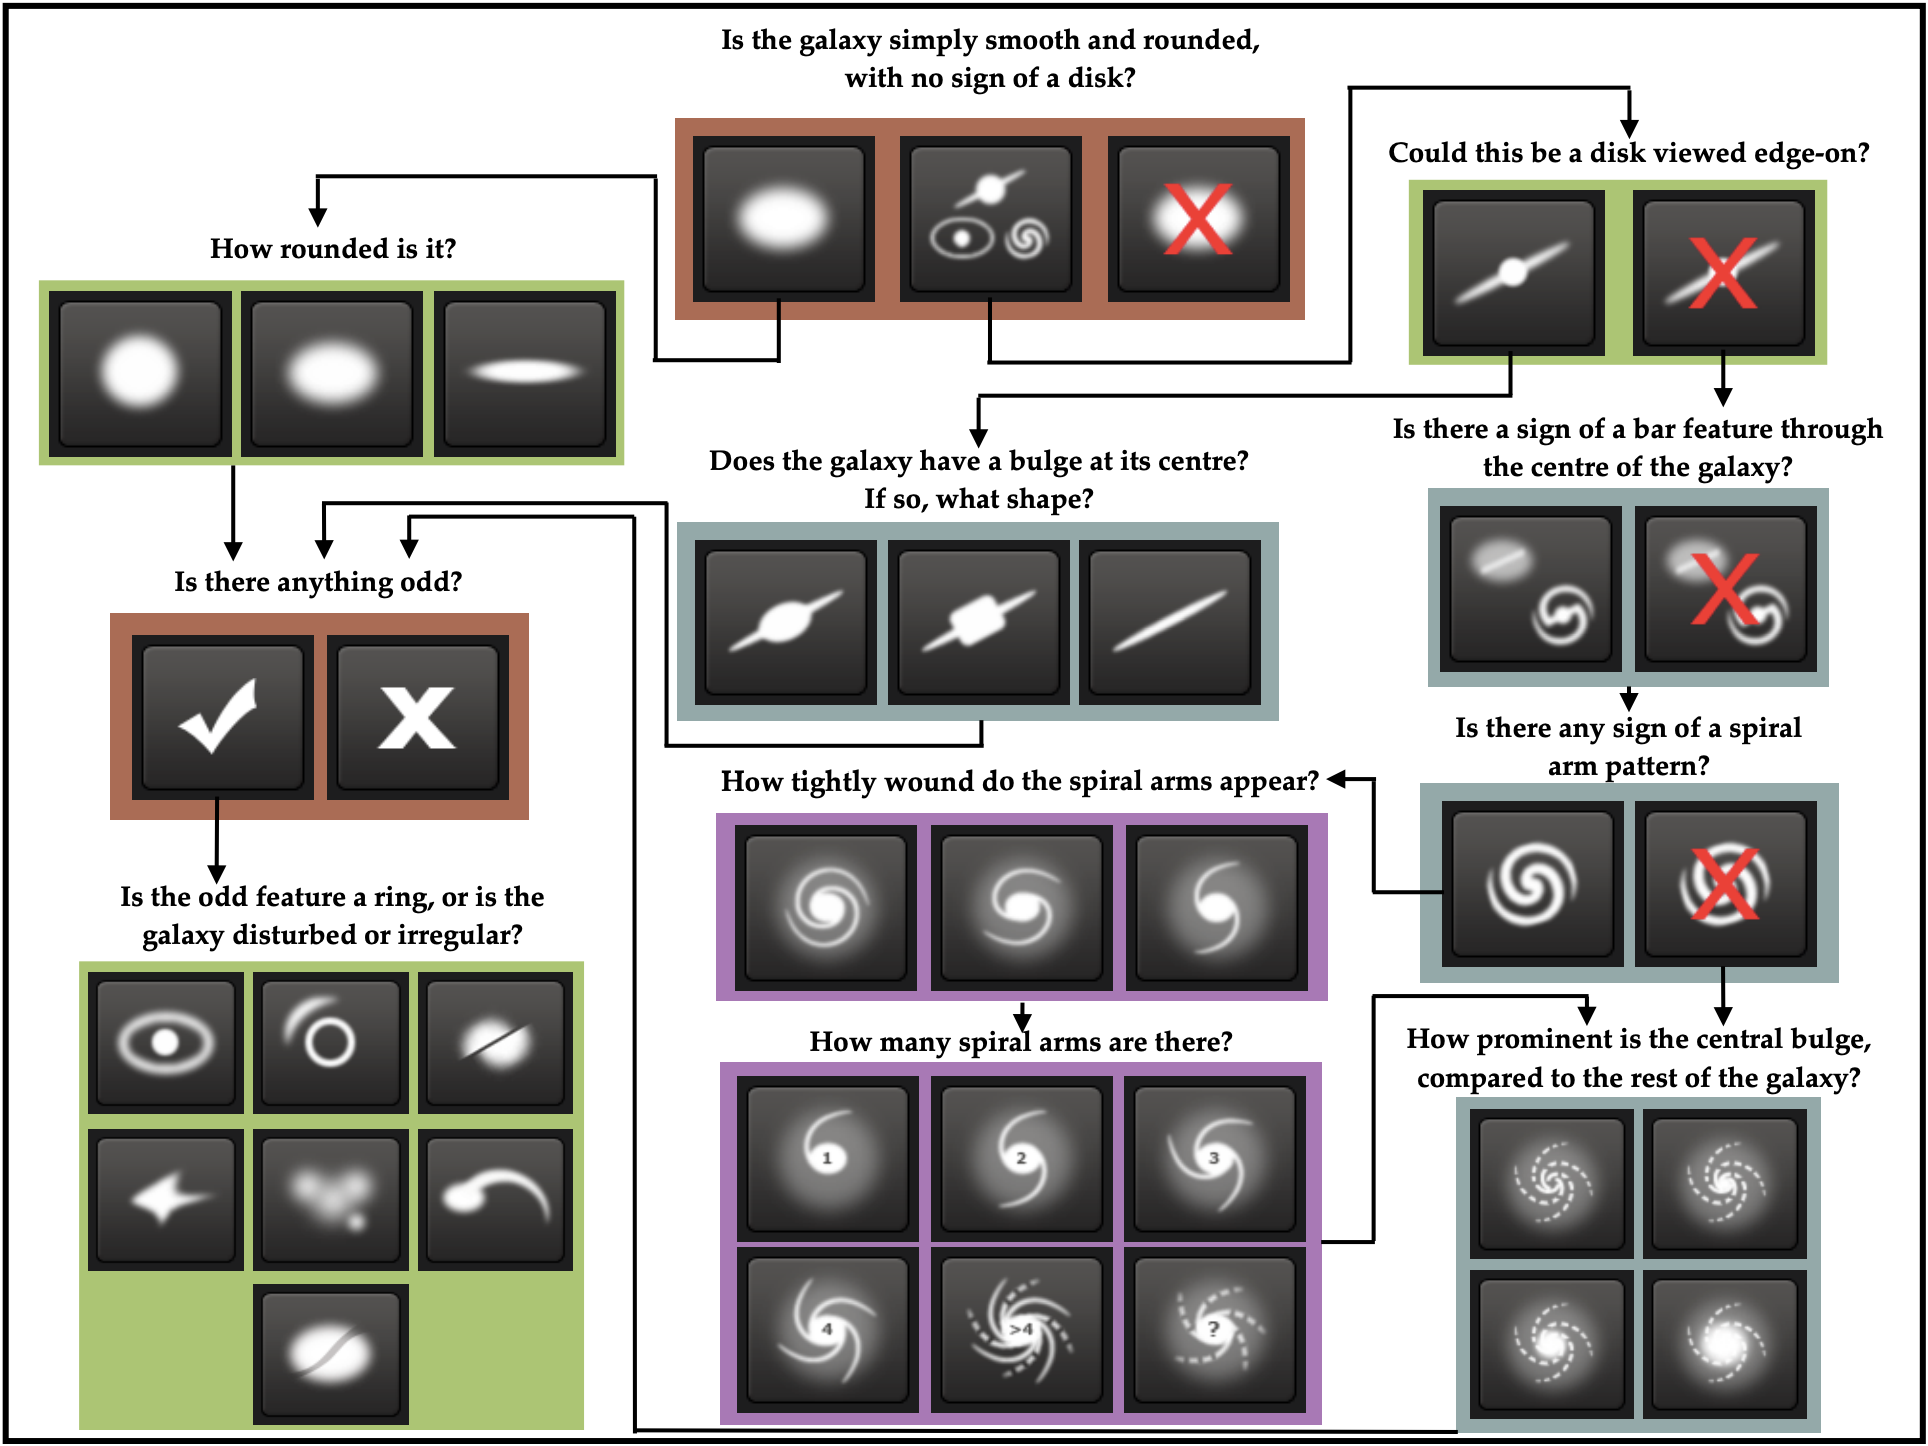
\includegraphics[width=\linewidth]{decision_tree.png}
    \caption{Image representation of the Galaxy Zoo 2 decision tree from the official Galaxy Zoo 2 Data Release \cite{Willett13}.}
    \label{fig:decisiontree}
  \end{figure}

To provide a more hollistic perspective on Galaxy Zoo 2 (GZ2), we selected the Galaxy10 dataset to use directly in our algorithms.
The Galaxy10 dataset combines the original GZ2 data, which includes over 270,000 SDSS galaxy images, with additional images from the DESI Legacy Imaging Surveys (DECaLS), totalling over 440,000 images.
The Galaxy10 dataset minimised class imbalance by merging the data into 10 broader classes and collectively sampling approximately 18,000 images from the SDSS and DECaLS data, offering a more even class distribution.
\begin{figure}[htbp]
    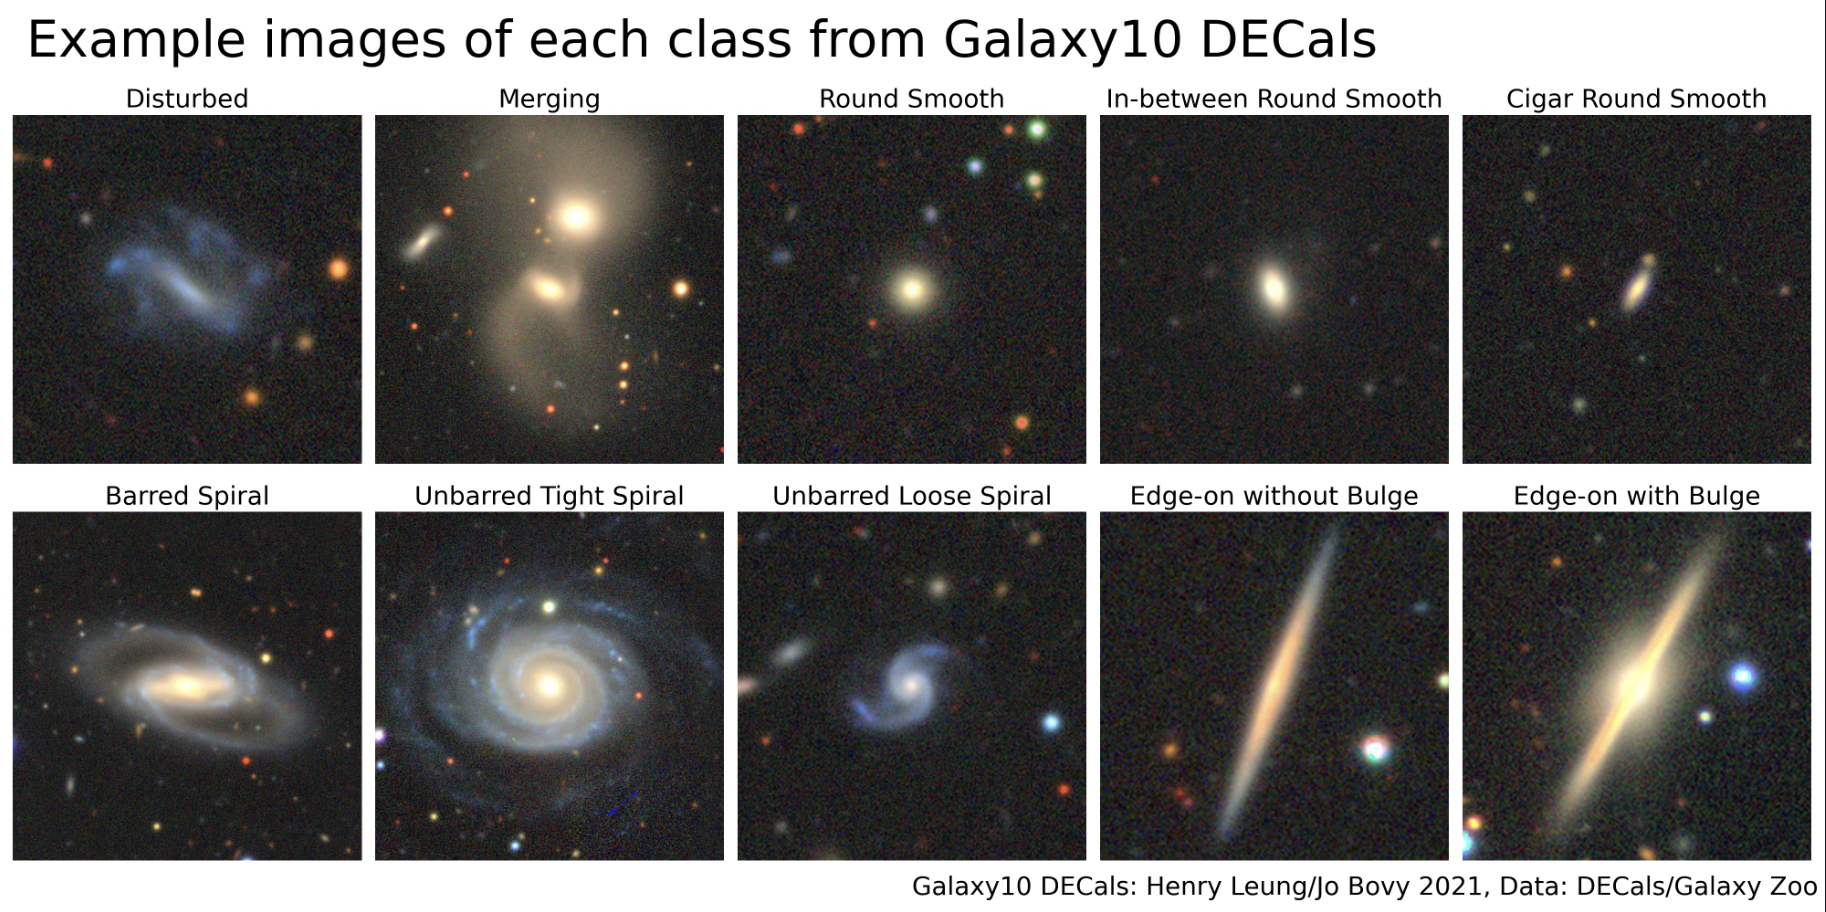
\includegraphics[width=\linewidth]{galaxy10_images.png}
    \caption{Example images from each class in Galaxy10 DECaLS. Taken from the official \href{https://astronn.readthedocs.io/en/latest/galaxy10.html}{Galaxy10 documentation}.}
    \label{fig:galaxyimgs}
  \end{figure}
  \begin{figure}[htbp]
    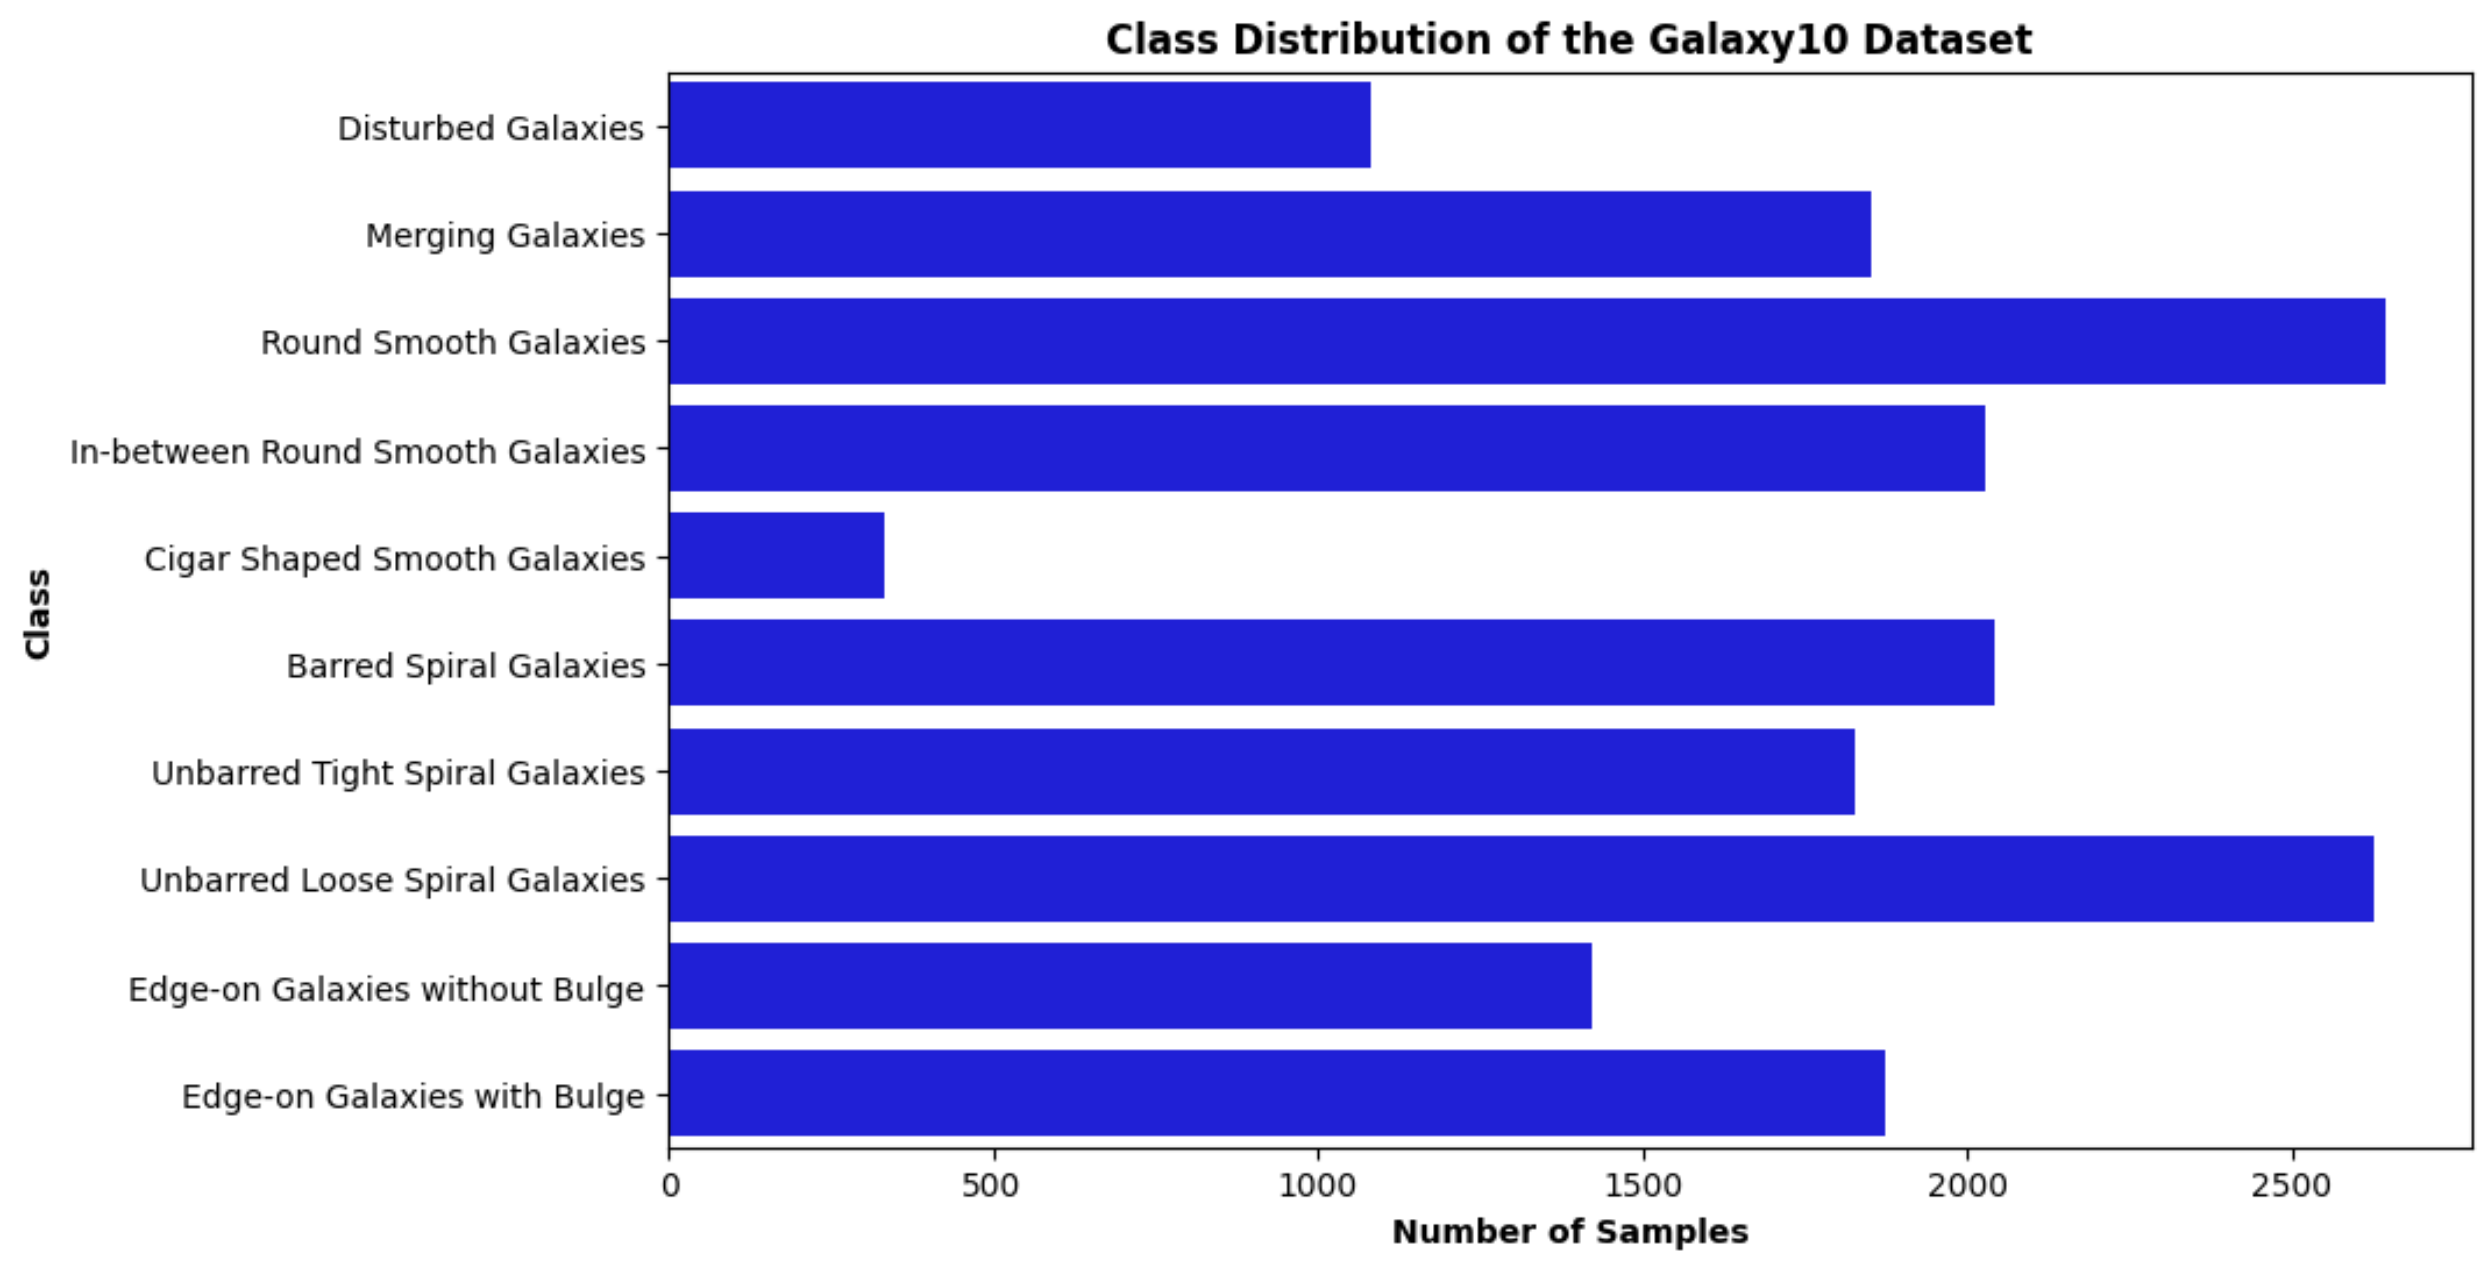
\includegraphics[width=\linewidth]{galaxy_distribution2.png}
    \caption{Class distribution in the Galaxy10 dataset.}
    \label{fig:featuredist2}
  \end{figure}

  \noindent The most frequent class, \textit{Round Smooth Galaxies}, contains 2,645 images and the least frequent class, \textit{Cigar Shaped Smooth Galaxies}, contains 334 images.
While this distribution is much more even than the Galaxy Zoo 2 dataset, the CNN model still faced significant difficulties in training due to the relatively smaller number of examples in some classes, which will be detailed in this paper.


\subsection{CNN Training on the Galaxy10 DECaLS Dataset}
Prior to generating artificial galaxy images using the cGAN, we trained the CNN on the original Galaxy10 dataset.
For smoother model training, we used the PyTorch library to construct our Convolutional Neural Network.
The network contained three 2D convolutional layers with 32, 64 and 128 filters, respectively, each followed by a pooling layer and, finally, a dense fully-connected layer containing 512 neurons.
This architecture was chosen for its simplicity and reliability in training. 
We wanted to avoid building deep architectures for the CNN in order to reduce runtime and better evaluate the effectiveness of the cGAN's artificial data generation on the model's performance. 

% % might need to delete this later for space
% \begin{figure}[htbp]
%     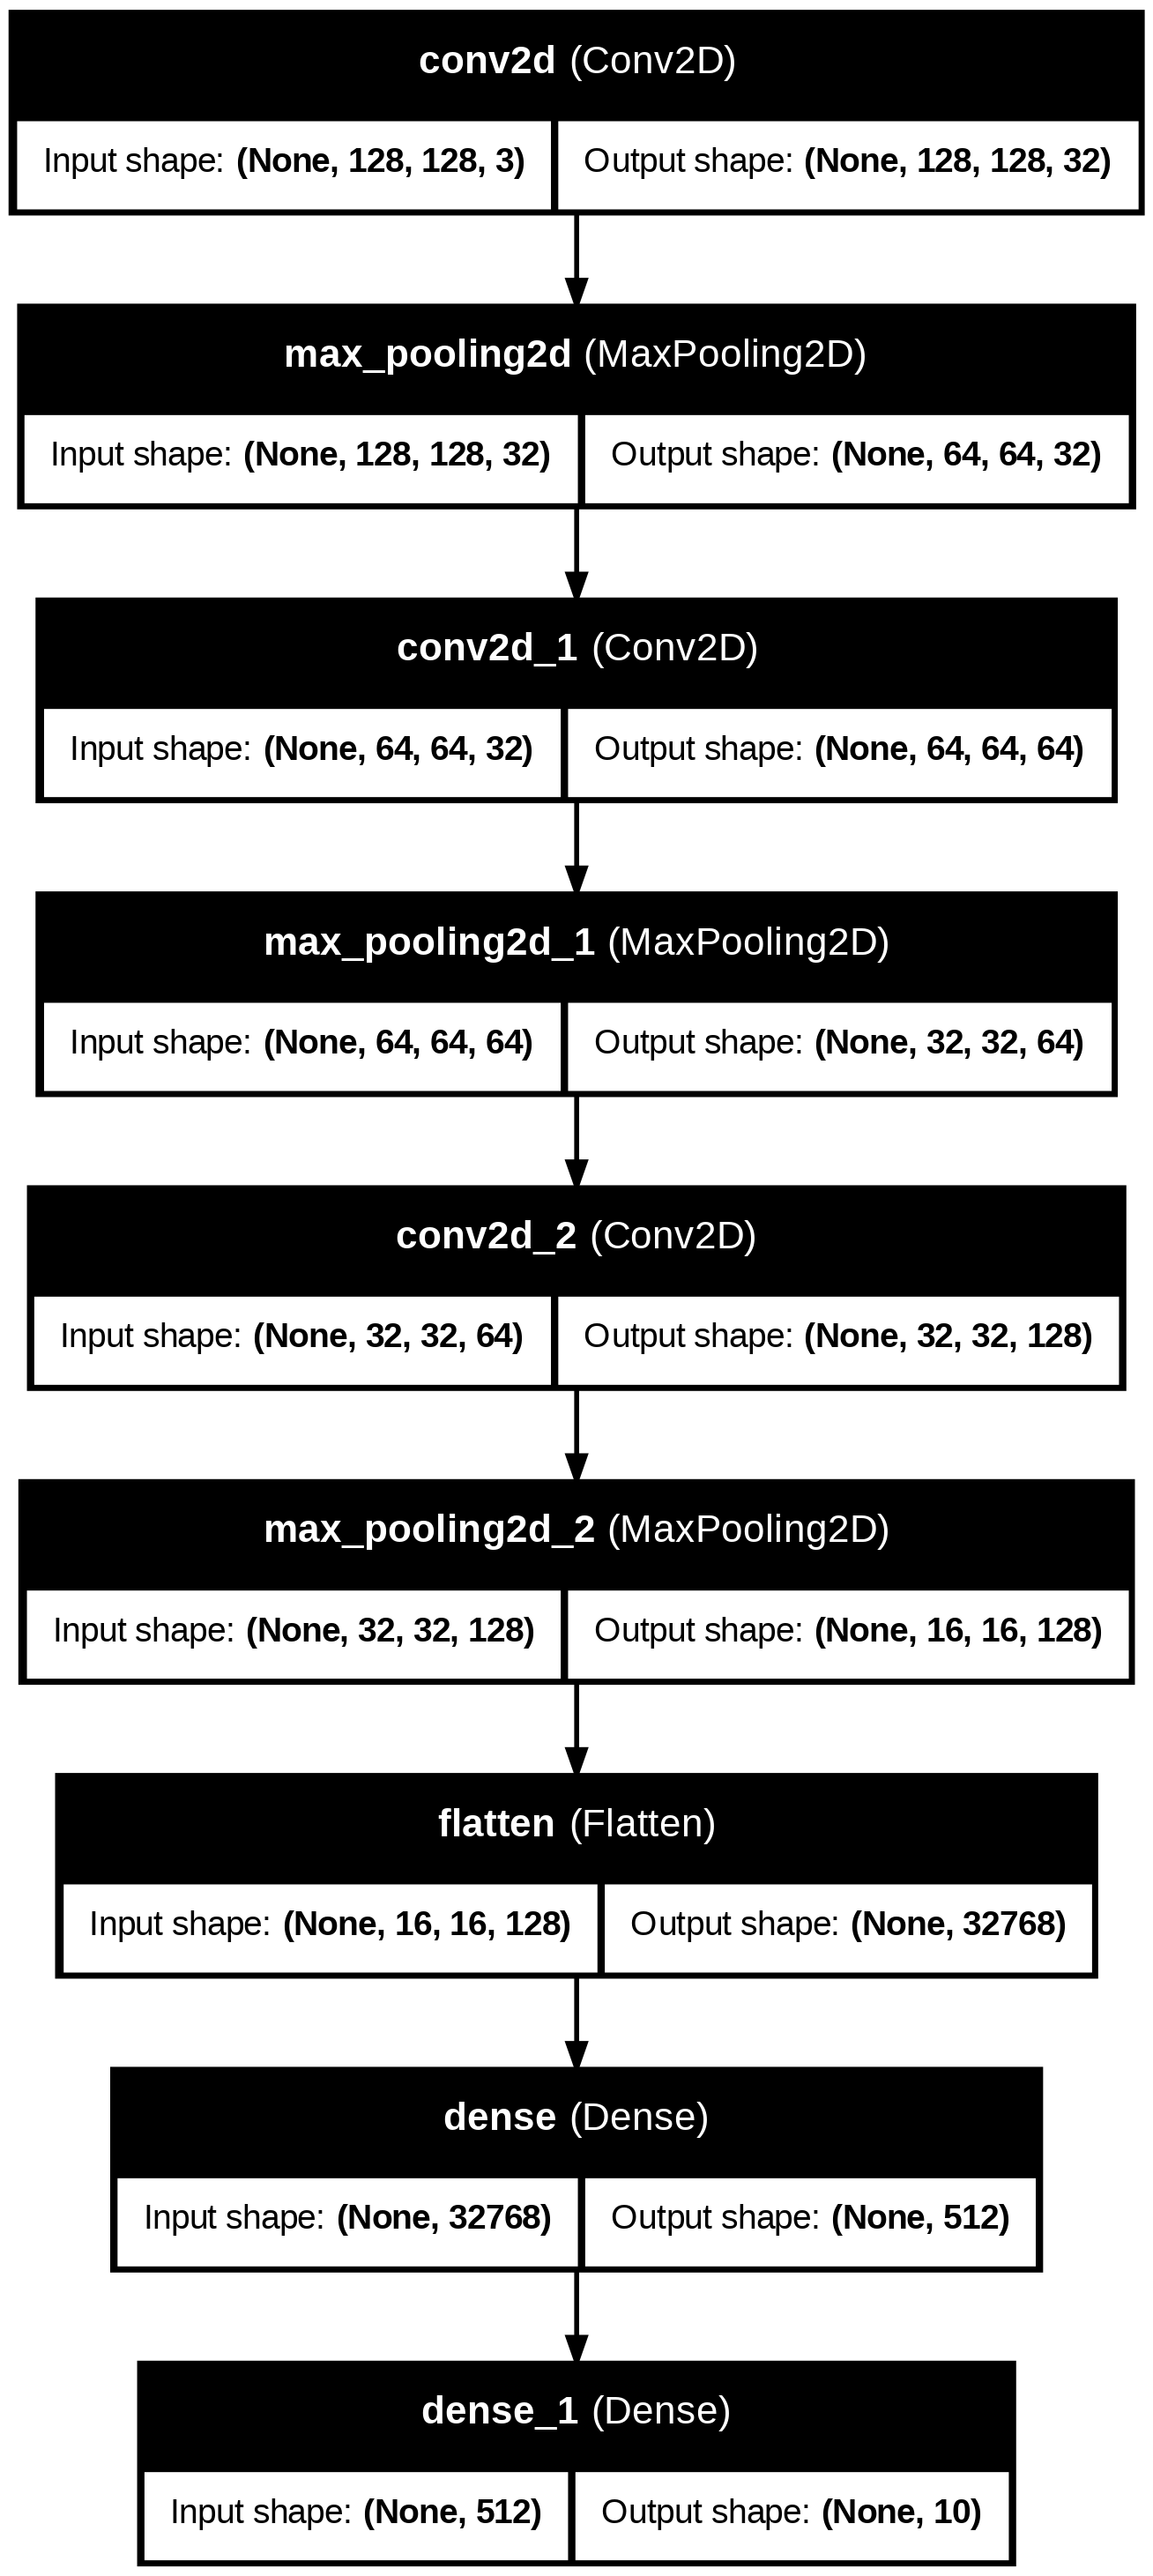
\includegraphics[width=\linewidth]{cnn_arch.png}
%     \caption{CNN architecture. Generated using Keras library.}
%     \label{fig:cnnarch}
%   \end{figure}


\subsection{Image Enhancement Using SRGAN}
The first task required in generating the synthetic galaxy images is to enhance their quality by implementing a Super-Resolution Generative Adversarial Network.
We ran the SRGAN on 100 epochs, producing upscaled images with improved resolution to better capture the fine details crucial for accurate classification.
The final SRGAN hyperparameters were tuned to contain 8 generator layers and 9 discriminator layers, which provided optimal high-resolution image enhancement without introducing additional artifacts.


\subsection{Synthetic Data Generation Using cGAN:} 
Before training and generating synthetic images using the Conditional Generative Adversarial Network, we had to identify which underrepresented classes to generate.
Classes containing less than 1,500 (placeholder) samples were labelled as "underrepresented" in the model, which put the \textit{Cigar Shaped Smooth Galaxies}, \textit{Disturbed Galaxies} and \textit{Edge-on Galaxies with Bulge} classes in such category.
The cGAN was then conditioned on these class labels, ensuring that the synthetic images resembled galaxies of the classes' specific morphological types. 

The first component of the cGAN is the generator, which was conditioned on the underrepresented classes and produced images that reseble the real images in that class.
The second component is the discriminator, whose task was to determine the probability a given image is real or fake.
The cGAN was trained on a learning rate of 0.0002 (placeholder) and batch size of (batch size) ultimately produced the best results and allowed the CNN to most effectively learn from a uniform distribution of galaxy characteristics.

% ADD GENERATED IMAGE EXAMPLES HERE
% ADD NEW CLASS DISTRIBUTION HERE

\subsection{GAN-CNN Pipeline Integration} 
Once we had obtained the generated synthetic images from the cGAN and the SRGAN-enhanced real images of the original dataset, the data was merged and used to re-train the CNN.



% Results
\section{Results}
\subsection{CNN Training on Original Dataset}
The CNN model was trained on both the original and augmented datasets to evaluate its ability to classify galaxy images. 
To compare the performance, we measured the accuracy, precision, recall and F1-score across both the original and augmented datasets.

When the CNN was trained on the original dataset, the training accuracy was significantly higher than the testing accuracy, reaching 99.29\% by the 10th epoch, while testing accuracy dropped from a maximum of 57.44\% during the 3rd epoch to 48.59\% during the 10th epoch.
A similar dip in performance can be seen in Figure 5, where the model was evaluated using precision, recall and F1-score metrics. 
The results are indicative of the class imbalance mentioned previously, with the network learning instances of the majority classes very well and failing to effectively categorise underrepresented classes. 
\begin{figure}[htbp]
    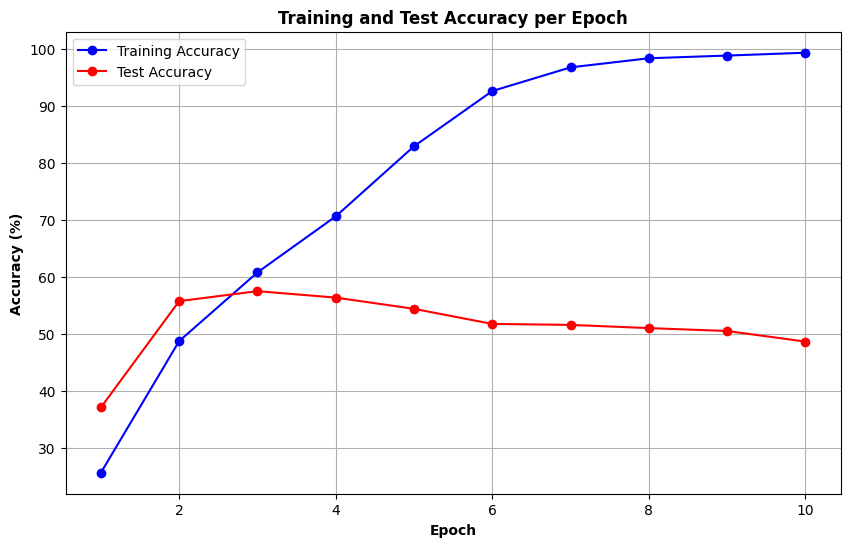
\includegraphics[width=\linewidth]{initial_cnn_acc.png}
    \caption{CNN performance on the original Galaxy10 dataset. Evaluated using training and testing accuracy.}
    \label{fig:initialcnnacc}
  \end{figure}
\begin{figure}[htbp]
    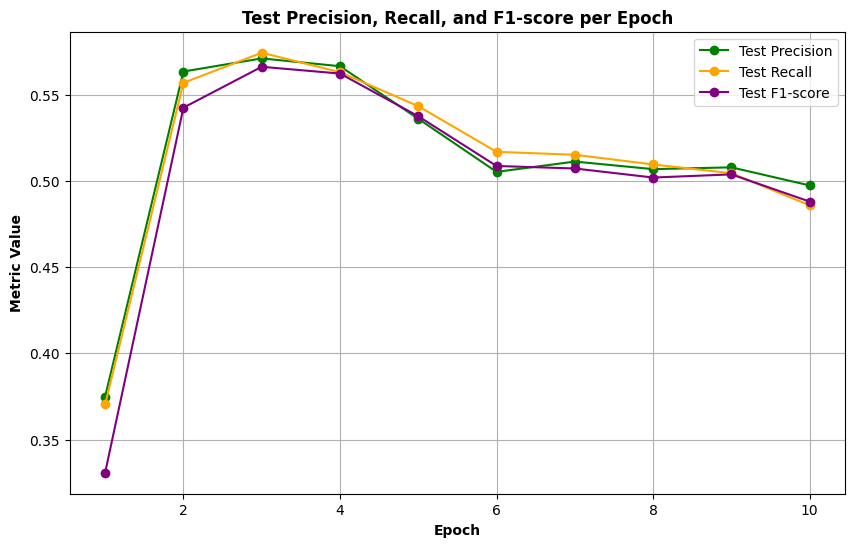
\includegraphics[width=\linewidth]{initial_cnn_metrics.png}
    \caption{CNN performance on the original Galaxy10 dataset. Evaluated using precision, recall and F1-score metrics.}
    \label{fig:initialcnnmet}
  \end{figure}


\subsection{Evaluation of SRGAN-Enhanced Images}
The SRGAN model was trained to upscale images by a factor of 2x. 
Visual inspection of the upscaled images showed noticeable improvements in clarity and detail, especially in smaller galaxy structures. 
We achieved an average PSNR value of 24.5 across the upscaled images, indicating a high degree of similarity between the generated high-resolution images and their lower-resolution counterparts.
\begin{figure}[htbp]
    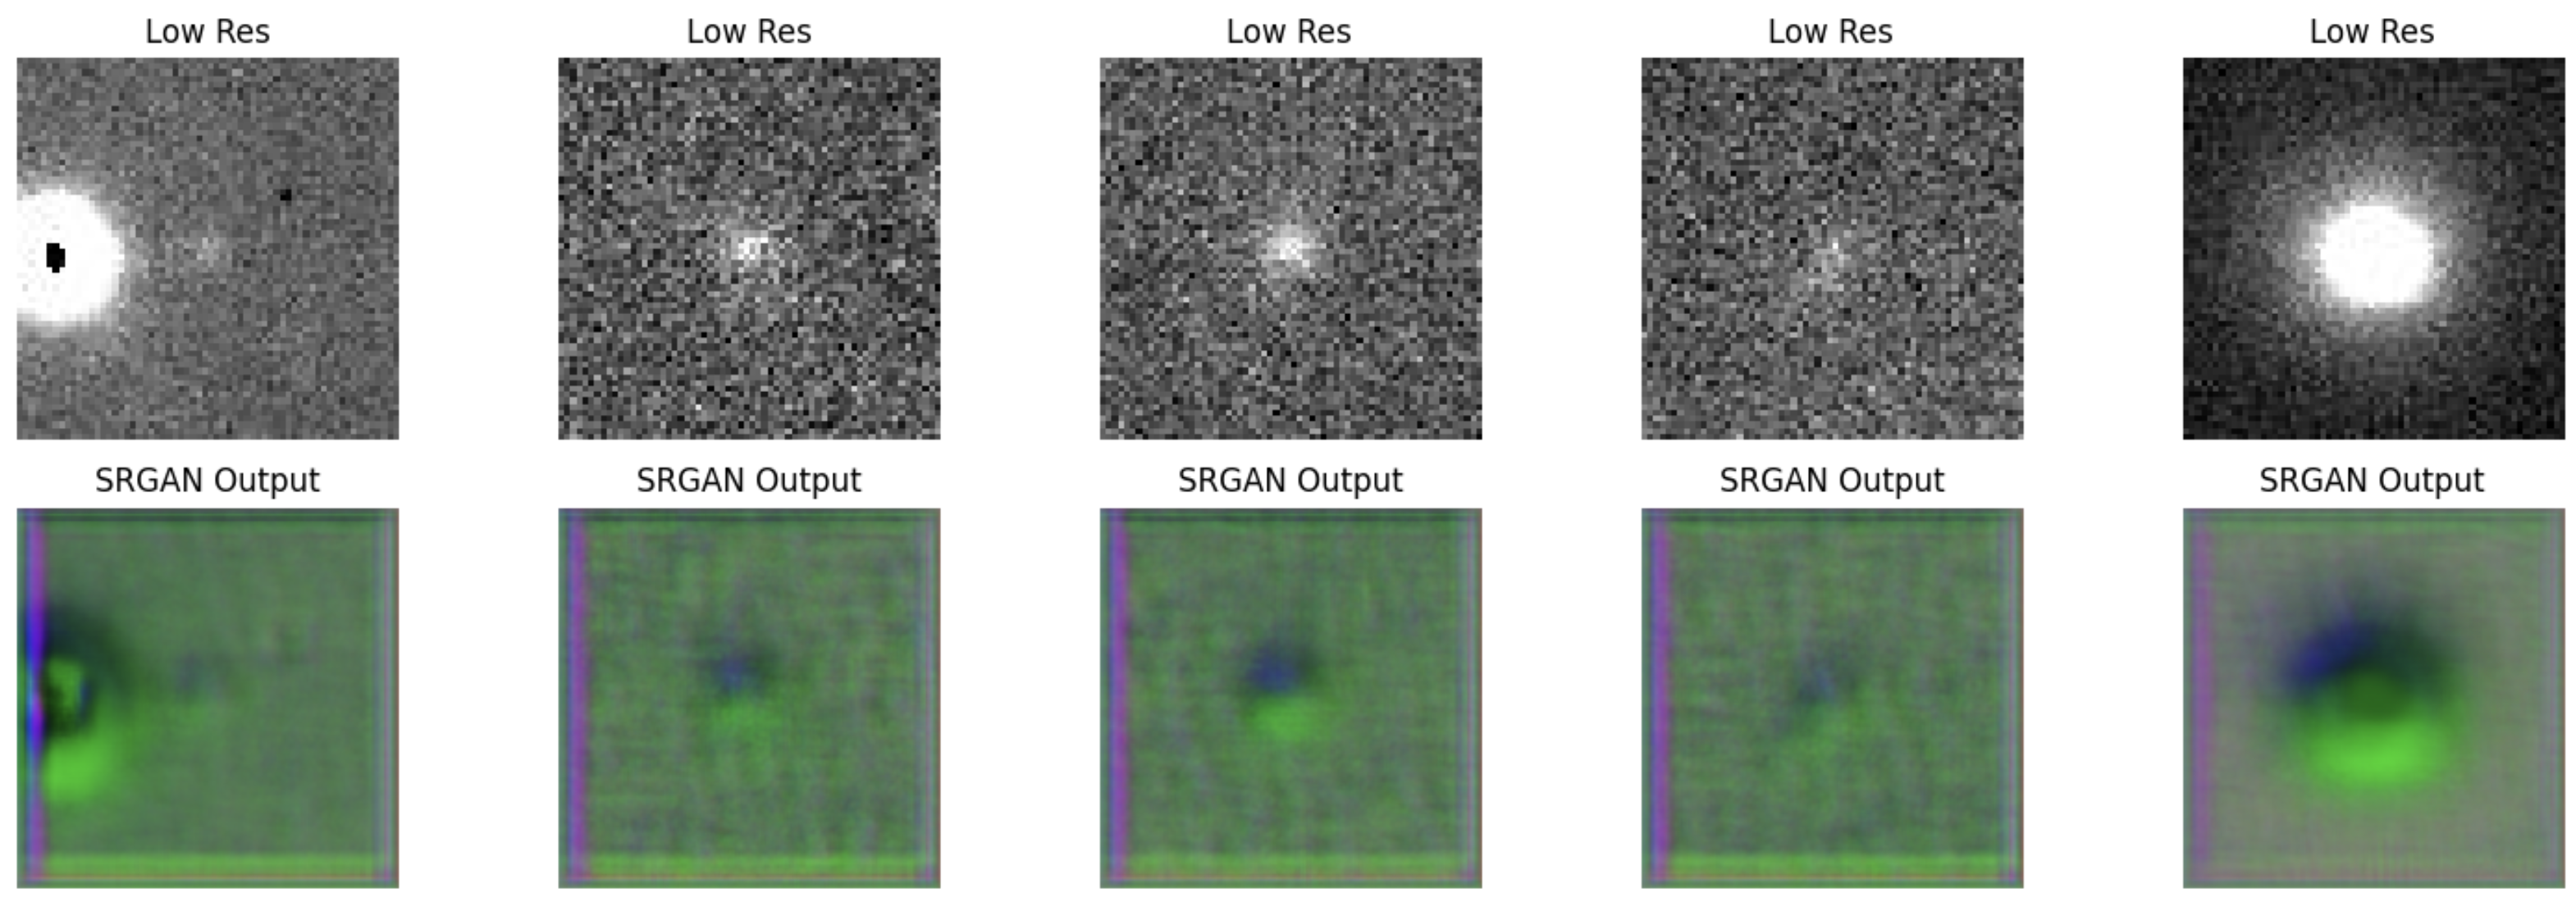
\includegraphics[width=\linewidth]{srgan.png}
    \caption{Galaxy images in low resolution and upscaled using SRGAN.}
    \label{fig:galaxysrgan}
  \end{figure}


\subsection{Qualitative Evaluation of cGAN-Generated Images}
% ADD PHOTOS AND LOSS (?)


\subsection{CNN Training on Augmented Dataset}
% ADD NEW ACCURACY AND EVALUATION METRICS RESULTS AND GRAPHS
% COMPARISON


% Conclusions
\section{Conclusion}

{
    \small
    % Include all references in the bibliography
    \nocite{*}
    \bibliographystyle{ieeenat_fullname}
    \bibliography{main}
}


\end{document}
